84. \begin{figure}[ht!]
\center{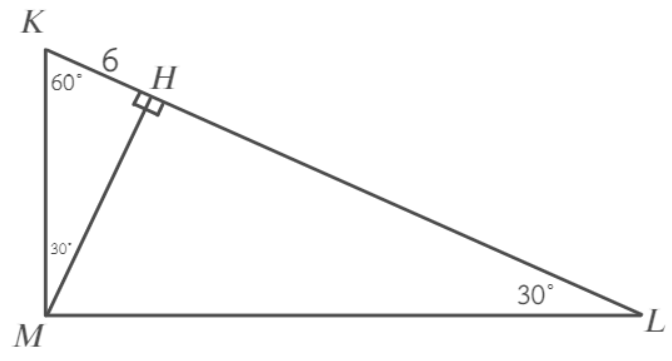
\includegraphics[scale=0.35]{g84.png}}
\end{figure}\\
Найдём $\angle KMH=90^\circ-60^\circ=30^\circ,\ \angle L=90^\circ-60^\circ=30^\circ.$ По теореме о катете, лежащем напротив угла в $30^\circ,$ для треугольников $MKH$ и $KML$ имеем $KM=2\cdot6=12,\ KL=2\cdot12=24.$ Тогда $LH=KL-KH=24-6=18.$
ewpage

oindent85. \begin{figure}[ht!]
\center{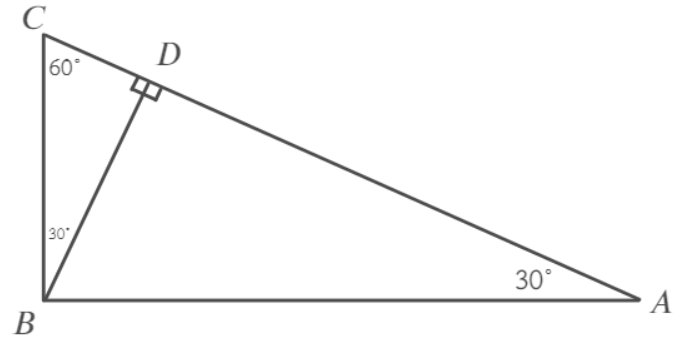
\includegraphics[scale=0.35]{g85.png}}
\end{figure}\\
В прямоугольном треугольнике $BCD$ катет $DC$ в 2 раза меньше гипотенузы $BC,$ значит $\angle CBD=30^\circ,\ \angle C=90^\circ-30^\circ=60^\circ,\ \angle A=90^\circ-60^\circ=30^\circ.$ Тогда по теореме о катете, лежащем напротив угла в $30^\circ,$ для треугольников $BCD$ и $ABC$ имеем $BC=2CD,\ AC=2BC=4CD,\ AD=AC-CD=3CD.$ Значит, отношение равно $3CD:CD=3:1.$\\
